\chapter{Simulation on multi-core computers}
In addition to the sequential Simulator class, \adevs\ has a ParSimulator class that is designed specifically to take advantage of processors that have multiple cores and shared memory machines with several processors, these possibly having several cores each. The parallel simulator is in most respects identical to the sequential simulator, and this section of the manual therefore focuses on where it is different.

The ParSimulator class is designed specifically (only, really) to support symmetric, shared memory multiprocessors (SMPs). The multi-core processors that have become ubiquitous in recent years are an important instance of this class of machines. The software technology that underlies the ParSimulator is OpenMP (see \url{http://www.openmp.org}), which is a standardized extension for C and C++ compilers and runtime systems to support multi-threaded computing. The OpenMP standard is now support by most (probably all) major compilers: the GNU C++ Compiler and professional editions of Microsoft Visual Studio are important examples (important to me, that is, because those are what I use for most of my simulation work).

The critical first step, therefore, to using the ParSimulator is to enable the OpenMP extensions for your compiler. For the GNU C++ compiler, simply add the flag '-fopenmp' to your linker and compiler arguments. For MS Visual Studio, this is a build option (though I forget the location of the switch, and do not at the moment have access to the professional edition). For other compilers and development environments, see your documentation. Prior to executing a simulation, the maximum number of threads that will be used by OpenMP (and, therefore, the simulator) can be set by setting the OMP\_NUM\_THREADS environment variable (this works for the GNU compilers, at least). The default in most cases is to use a number of threads equal to the number of processors or cores in your computer.

Having enabled the OpenMP options for your compiler, you are ready to start preparing your model to work with the parallel simulator. As a first step, you can do the following. This example assumes that your main simulation routine looks something like this:
\begin{verbatim}
...
Simulator<IO_Type>* sim = new Simulator<IO_Type>(my_model);
/**
 * Register listeners with the Simulator to collect statistics
 * ....
 */
while (sim->nextEventTime() < t_end)
    sim->execNextEvent();
...
\end{verbatim}
or this
\begin{verbatim}
...
Simulator<IO_Type>* sim = new Simulator<IO_Type>(my_model);
/**
 * Register listeners with the Simulator to collect statistics
 * ....
 */
sim->execUntil(t_end);
...
\end{verbatim}
which does the same thing. The reason for this assumption is described in the section on limitations. Note, however, that any Listeners you have registered with your Simulator instance will work normally )almost, I'll get to that).

Assuming you have code like the above, replace it with code like the following:
\begin{verbatim}
...
ParSimulator<IO_Type>* sim = new ParSimulator<IO_Type>(my_model);
/**
 * Register listeners with the ParSimulator to collect statistics
 * ....
 */
sim->execUntil(t_end);
...
\end{verbatim}
This should work just like your previous code with the following caveats.

First, your models must not share variables; all information exchanged between models must occur via events at their input and output. Also note that the order of items in the bags of input received by your model may change from run to run, though the contents are guaranteed to be the same. Therefore, the repeatability of your simulation runs depends on your models being insensitive to the order of elements in their input bags.

Second, reports produced by your listeners may be formatted in ways you do not expect: for any individual atomic model, the listing of state transitions and output events will be in time order. Across models, however, this may not be the case. For an extreme example, suppose that you have two atomic models arranged as follows: A->B. You may see all state transitions and output for A listed first, followed by all state transitions and outputs for B. Most likely, these will be intermingled. Note too that the output reported for network models may not be in its proper time order, though the output reported for its atomic components will be.

This latter effect is due to the fact that, while simulation of each model is done in the proper time order of its events, the ParSimulator overlaps simulation of models whenever this is possible. In the above example, it is possible to simulate model A without worrying about what B is doing because B never provides input to A. The simulator (if properly configured, as is described next) will take advantage of this to simulate A and B in parallel. Hence, we may see all of the output from A before we see anything for B. Once again, however, all callbacks to registered Listeners for any particular model will be in the proper time order.

Note too that this implies that callbacks to your listeners may occur in parallel. In the above example, it may be that the same listener receives concurrent notifications about a state change for model A and state change for model B, or output from A and state change of B, or any such combination. It is imperative therefore that the callbacks in your listeners be thread safe.

This implies also that your network models must have routing methods that are thread safe. This is the case for the network models that are included with adevs. If you have implemented your own network models, be sure that their route methods are thread safe as well.

Third, and most critical, your atomic components must implement the new lookahead method, which is inherent from the Devs base class. This method must return a positive value subject to the guarantees described in the next section on ``Principles of the parallel simulator''. For the purposes of getting your code to compile and run, your lookahead methods can simply return a very small value (i.e., something positive but close to zero; say 1E-8 or 1E-9). In this case, your simulator should compile and (very slowly) execute. Even if you have the patience to wait for it to complete, however, the outcome will likely be wrong. Nonetheless, such a test will let you get your build environment setup properly.

The above changes are sufficient in most cases to make your existing, sequential simulator execute with the parallel simulator. In summary, these mandatory steps are:
\begin{enumerate}
\item Replace your Simulator with a ParSimulator.
\item Use the ParSimulator's execUntil method to advance time.
\item Make sure your Listeners are thread safe.
\item Make sure your Networks' route methods are thread safe.
\item Implement the lookahead method for your Atomic models.
\end{enumerate}

These steps alone are unlikely to yield an improvement in performance (or, indeed, correct results). As a general rule, correctly speeding up your simulation requires that the ParSimulator be given specific information about your model; information that only you can provide. Without this information, the synchronization overhead incurred by the parallel simulation algorithm is staggeringly huge. The majority of this document deals with the problem of creating fast and correctly executing simulations.
 
\section{Limits of the parallel simulator}
Before continuing any effort to make your simulator work with the algorithms used by the ParSimulator, you should be aware of specific capabilities of the sequential simulator that the parallel simulator does not support. These are:
\begin{enumerate}
\item Your compiler must support OpenMP.
\item The execNextEvent, computeNextState, and computeNextOutput methods are not provided. Only the execUntil method is provided for advancing the simulation.
\item As noted above, callbacks to a Listener for each individual atomic model will be given in the proper time order, but these may be arbitrarily interleaved with the callbacks for other atomic models.
\item Listener callbacks must be made thread safe using the OpenMP synchronization features.
\end{enumerate}

Beyond these purely technical limits, it should be noted that making effective use of this (or any) parallel discrete event simulator is often difficult. Applications of practical interest require the identification of lookahead for the model's atomic components (described in the next section), partitioning of the model amongst the available processors, and implementing code to enable the parallel simulator to take advantage of your model's lookahead and partitioning.

So while this guide addresses issues specific to using the adevs ParSimulator class, I strongly recommend that, if you are not already intimately familiar with parallel simulation, that you obtain a book on the topic. ``Building Software for Simulation'', authored by James Nutaro (the author of this manual) and published by Wiley in 2011, contains a chapter on conservative discrete event simulation with DEVS in general and adevs in particular. You may find this book to be a useful introduction, though there are other excellent texts on the subject.

\section{Modifying your models to exploit lookahead}
The ParSimulator takes advantage of a property intrinsic to many models: their strong causality. A model, network or atomic, is strongly causal if its output can be predicted with certainty to some future time without knowledge of its input. The length of time into the future for which this prediction can be made is called lookahead.

To illustrate, consider a very simple, atomic model that acts as follows. In the absence of input, the model neither changes state nor produces output: its time advance is infinite. Upon receiving an input, the model retains it for exactly one unit of time and then expels it. So, for example, if the input to the system is the series of letters 'A', 'B', and 'C' at times 1, 2, and 3 respectively, the its output comprise 'A', 'B', and 'C' at times 2, 3, and 4 respectively. If the model receives an input while in the process of transcribing, then that input is discarded. So, for example, if 'A', 'B', and 'C' arrive at times 2, 2.5, and 3 then the output from the model is 'A' and 'C' at times 3 and 4.

Now observe that if I know the input to this model until some time t, then I can determine its output until time t+1 and, to do this, I do not need to know its input in the interval from t to t+1. For instance, suppose I know that the input at time zero is 'A'. Clearly, the only output of the model in the interval 0 to 1 (inclusive) is the value 'A' at time 1. Moreover, suppose I know that the input at t=0 is 'A' and that there is no other input until at least time 0.5. In this case, I know that the output until (but not including) time 1.5 consists only of 'A' at time 1. Any input following time 0.5 cannot occur until, at its earliest, time 1.5. This model has a lookahead of 1. Given its input to time t, its output is fixed to time t+1. Output in this interval does not depend on input in the same interval.

In network models, lookahead may accumulate. As an example, suppose that two transcribers are connected in series. In this case, the lookahead of the composite is two; i.e., the sum of the lookaheads of the components. If, however, a network model comprises two transcribers in parallel, then the lookahead of the network is only one. Generally speaking, however, larger networks tend to have larger lookaheads, and large lookahead is essential for getting good performance from the simulator.

To take advantage of lookahead in a model, the simulator must be told that it exists. This is done by overriding the lookahead method of the Devs class. All atomic and network models inherit this method from the Devs base class, and its default implementation is to return zero. 

Lookahead is most useful to the simulator if it is coupled with a capability to actually calculate the model's outputs to this time. To calculate those outputs, however, requires knowledge of the intervening states. An atomic model enable the simulator to project its output into the future by implementing two method: beginLookahead and endLookahead.

The beginLookahead method is called to notify the model that further calculations of its outputs and state transitions are speculative. The default behavior of the beginLookahead method is to throw an exception, which notifies the simulator that this model does not support the projection of its output into the future. An atomic model overriding this method must be capable of restoring its state variables to their follows at the instant that beginLookahead was called. The endLookahead method is called by the simulator when it is done projecting that model's output. This method must restore the model to the same state it was in when the beginLookahead method was called.

These methods are demonstrated by the Transcribe class shown below. This atomic model implements the transcriber described above.
\begin{verbatim}
/**
 * This model copies its input to its output following a
 * delay.
 */
class Transcribe:
	public adevs::Atomic<char>
{
	public:
		Transcribe():adevs::Atomic<char>(),ttg(DBL_MAX),to_transcribe(' '){}
		void delta_int() { ttg = DBL_MAX; }
		void delta_ext(double e, const adevs::Bag<char>& xb)
		{
			if (ttg == DBL_MAX)
			{
				ttg = 1.0;
				// Find the largest input value
				adevs::Bag<char>::const_iterator iter = xb.begin();
				to_transcribe = *iter;
				for (; iter != xb.end(); iter++)
				{
					if (to_transcribe < *iter)  to_transcribe = *iter;
				}
			}
			else ttg -= e;
		}
		void delta_conf(const adevs::Bag<char>& xb)
		{
			delta_int();
			delta_ext(0.0,xb);
		}
		void output_func(adevs::Bag<char>& yb)
		{
			yb.insert(to_transcribe);
		}
		double ta() { return ttg; }
		void gc_output(adevs::Bag<char>&){}
		double lookahead() { return 1.0; }
		void beginLookahead()
		{
			// Save the state
			chkpt.ttg = ttg;
			chkpt.to_transcribe = to_transcribe;
		} 
		void endLookahead()
		{
			// Restore the state
			ttg = chkpt.ttg;
			to_transcribe = chkpt.to_transcribe;
		} 
		char getMemory() const { return to_transcribe; }
	private:
		double ttg;
		char to_transcribe;
		struct checkpoint_t { double ttg; char to_transcribe; };
		checkpoint_t chkpt;
};
\end{verbatim}

A model comprising two transcribers connected in series could be defined as follows. Note that this network model does not have the endLookahead and beginLookahead methods. State is a property of atomic models only, and therefore only atomic models may implement these methods.
\begin{verbatim}
/**
 * This model defines a pair of transcribers connected
 * in series as shown: -> t1 -> t2 ->.
 */
class Series:
	public adevs::Network<char>
{
	public:
		Series():
			Network<char>(),
			t1(),t2()
		{
			t1.setParent(this);
			t2.setParent(this);
		}
		void getComponents(adevs::Set<adevs::Devs<char>*>& c)
		{
			c.insert(&t1);
			c.insert(&t2);
		}
		void route(const char& x, adevs::Devs<char>* model,
			adevs::Bag<adevs::Event<char> >& r)
		{
			adevs::Event<char> e;
			e.value = x;
			if (model == this) e.model = &t1;
			else if (model == &t1) e.model = &t2;
			else if (model == &t2) e.model = this;
		}
		double lookahead()
		{
			return t1.lookahead()+t2.lookahead();
		}
	private:
		Transcribe t1, t2;
};
\end{verbatim}

The above code examples illustrate all possible changes of your models - network and atomic - to facilitate parallel simulation. Of these changes, only the lookahead method of the atomic model is actually required. The ParSimulator calculates default (and very conservative) lookaheads for the Network models if these are required. Atomic models that provide the endLookahead and beginLookahead methods may improve the execution time of the simulation. But only the lookahead values of the atomic models (or their parents if the model is partitioned by hand; see the next section) are actually required for correct execution of your model.

\section{Partitioning your model}
Each thread in your simulator is assigned responsibility for the execution of a subset of the atomic components of your model. Models within a thread are executed sequentially. Simulation of the models within a thread proceeds just as with the sequential Simulator class. The threads execute in parallel, each stopping to synchronize with its neighbors only as necessary to exchange essential information.

In an ideal partitioning of the model, each thread is assigned roughly the same number of models, each model requires roughly the same amount of computational effort to simulate, and models assigned to separate threads exchange inputs and outputs rarely or not at all. This is the ideal that you should strive for in assigning your models to the threads of your simulation algorithm.

The actual assignment of a model to a thread is straightforward. Network and Atomic objects inherent the setProc method from their Devs base class. To assign the model to a particular thread, pass the number of that thread to the setProc method before the ParSimulator is created. Threads are numbered from 0 to the maximum number of threads (i.e., OMP\_NUM\_THREADS) minus one.

As the ParSimulator setups the simulation, it will examine the thread to which each model is assigned and take the following actions:
\begin{enumerate}
\item If the model's parent is assigned to thread k, then the model is also assigned to thread k, regardless of the argument passed to its setProc method.
\item If the model's parent was not assigned to specific thread, then the model will be assigned to the thread indicated by argument to its setProc method.
\item If neither the model nor its parent were assigned to a thread via the model's setProc method, then it is assigned to a thread selected at random.
\end{enumerate}

This partitioning of the model tells the simulator how to distribute its computational workload. It does not tell the simulator which parts of the workload talk to which others. For example, if half of your model is assigned to thread 0 and the other half to thread 1, the simulator does not yet know if the model's in 0 send input to the models in 1, vice versa, or both. Without further information, the simulator will therefore assume that every thread contains models that must communicate with all other threads. This is the most conservative assumption, and carries with it a substantial synchronization overhead.

If you know something about how the models assigned to the thread communicate, then you can provide this information to the simulator. This is done by passing and LpGraph object to the constructor of the ParSimulator. The LpGraph is nothing more than a directed graph, and the presence of an edge from node k to node j indicates that the models for thread k send input to the models in thread j. Absence of an edge indicates no flow of information along the missing edge. An edge is added by calling addEdge(A,B) to create an edge from thread A to thread B.

The following snippet of code illustrates the partitioning procedure. This segment of code creates the block diagram model shown in Fig. \ref{fig:partition_example}. This model consists of two atomic components, A and B, and a network with two components C1 and C2. The model A is assigned to thread 0, B to thread 1, and the network C with its components C1 and C2 to thread 2. With this partition, thread 0 sends input to thread 1, thread 1 sends input to thread 2, and thread 2 to thread 0. 
\begin{verbatim}
ModelA* A = new ModelA();
ModelB* B = new ModelB();
NetworkModelC* C = new NetworkModelC();
SimpleDigraph<IO_Type>* model = new SimpleDigraph<IO_Type>();
model.add(A);
model.add(C);
model.add(B);
model.couple(A,B);
model.couple(B,C);
model.couple(C,A);
A.setProc(0);
B.setProc(1);
C.setProc(2);
LpGraph lpg;
lpg.addEdge(0,1);
lpg.addEdge(1,2);
lpg.addEdge(2,3);
ParSimulator<IO_Type> sim(model,lpg);
\end{verbatim}
\begin{figure}[ht]
\centering
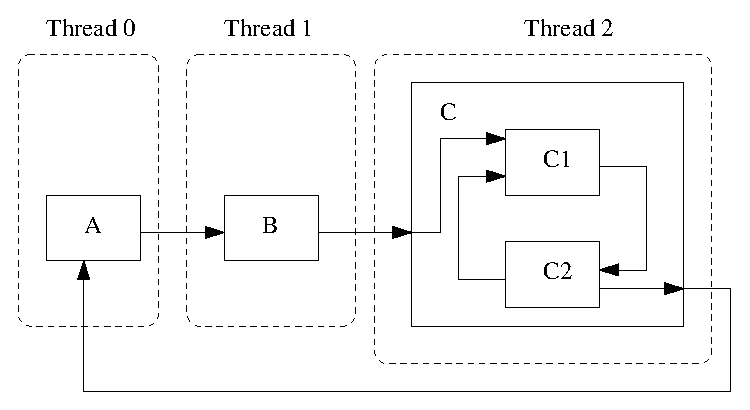
\epsfig{file=parsim_figs/partition_example.eps}
\caption{Partitioning a model for simulation on three processors.}
\label{fig:partition_example}
\end{figure}

\section{Interaction between partitioning and lookahead}
The following rules dictate which models must provide positive lookahead.
\begin{enumerate}
\item An atomic model whose parent is not assigned to a specific thread must provide a positive lookahead.
\item A network that is assigned to a specific thread, but whose parent is not, must provide a positive lookahead. 
\item No other model is required to provide a positive lookahead, or indeed any lookahead at all. The simulator will not use lookahead values provided by models except as indicated in cases 1 and 2 above.
\end{enumerate}

\section{A complete example}
This example builds and simulates the network shown in Fig. \ref{fig:partition_example} using the Transcribe model for components B, C1, and C2; a SimpleDigraph for the network C, and the following network for component A.

The network that is component A has two sub-components: a generator and a transcriber. Input to the network goes to the generator; output from the generator goes to the transcriber; and output from the transcriber becomes an output from the network. The generator operates as follows. It produces output at regular intervals of 1/2 units of time until it receives an input. At that time it stops. Note that the lookahead of the generator is zero because its pending output may be canceled at any time. The lookahead of the network, however, is one. That is, the lookahead of the network is the sum of its series components. 

A Listener is constructed for this model that records the state and output trajectories of every component. Observe two facts concerning the listener. First, it has been made thread safe by the critical section placed around writes to standard output. Second, it reports state and output trajectories for each atomic model in proper time order, but interleaves the trajectories of these models with each other. This second point will be apparent when we execute the simulation.

The complete implementation of the model, listener, and simulator are shown below.
\begin{verbatim}
#include "Transcribe.h"
#include "Genr.h"
#include "adevs.h"
#include <iostream>
using namespace adevs;
using namespace std;

/**
 * Extend the SimpleDigraph class to allow its lookahead
 * to be set manually.
 */
class SimpleDigraphWithLookahead:
	public SimpleDigraph<char>
{
	public:
		SimpleDigraphWithLookahead():
			SimpleDigraph<char>(),
			look_ahead(0.0)
			{
			}
		void setLookahead(double look_ahead)
		{
			this->look_ahead = look_ahead;
		}
		double lookahead() { return look_ahead; }
	private:
		double look_ahead;
};

/**
 * Listener to record the output and state trajectories of the
 * component models.
 */
Genr* A_g;
Transcribe *A_t, *B, *C1, *C2;
SimpleDigraphWithLookahead *A, *C;

class Listener:
	public EventListener<char>
{
	public:
		Listener(){}
		void outputEvent(Event<char> y, double t)
		{
			string which = which_model(y.model);
			#pragma omp critical
			cout << which << " @ t = " << t << ", y(t)= " << y.value << endl;  
		}
		void stateChange(Atomic<char>* model, double t)
		{
			if (model == A_g)
				#pragma omp critical
				cout << which_model(A_g) << " @ t = " << t << ", running= "
					<< A_g->isRunning() << ", next output= " <<
					A_g->getNextOutput() << endl;
			else if (model == A_t)
				#pragma omp critical
				cout << which_model(A_t) << " @ t = " << t << ", memory= "
					<< A_t->getMemory() << ", ta()= " <<
					A_t->ta() << endl;
			else if (model == C1)
				#pragma omp critical
				cout << which_model(C1) << " @ t = " << t << ", memory= "
					<< C1->getMemory() << ", ta()= " <<
					C1->ta() << endl;
			else if (model == C2)
				#pragma omp critical
				cout << which_model(C2) << " @ t = " << t << ", memory= "
					<< C2->getMemory() << ", ta()= " <<
					C2->ta() << endl;
			else if (model == B)
				#pragma omp critical
				cout << which_model(B) << " @ t = " << t << ", memory= "
					<< B->getMemory() << ", ta()= " <<
					B->ta() << endl;
			else assert(false);
		}
	private:
		string which_model(Devs<char>* model)
		{
			if (model == A_g) return "A.A_g";
			if (model == A_t) return "A.A_t";
			if (model == A) return "A";
			if (model == B) return "B";
			if (model == C1) return "C.C1";
			if (model == C2) return "C.C2";
			if (model == C) return "C";
			assert(false);
			return "";
		}
};

int main(int argc, char** argv)
{
	// Component A
	A_g = new Genr();
	A_t = new Transcribe();
	A = new SimpleDigraphWithLookahead();
	A->setLookahead(A_t->lookahead()+A_g->lookahead());
	A->add(A_g);
	A->add(A_t);
	A->couple(A,A_g); // A -> A_g
	A->couple(A_g,A_t); // A_g -> A_t
	A->couple(A_t,A); // A_t -> A
	A->setProc(0); // Assign to thread zero
	// Component B
	B = new Transcribe();
	B->setProc(1); // Assign to thread one
	// Component C
	C1 = new Transcribe();
	C2 = new Transcribe();
	C = new SimpleDigraphWithLookahead();
	C->setLookahead(C1->lookahead()+C2->lookahead());
	C->add(C1);
	C->add(C2);
	C->couple(C,C1); // C -> C1
	C->couple(C2,C); // C2 -> C
	C->couple(C1,C2); // C1 -> C2
	C->couple(C2,C1); // C2 -> C1
	C->setProc(2); // Assign to thread two
	// Create the overarching model
	SimpleDigraph<char>* model  = new SimpleDigraph<char>();
	model->add(A);
	model->add(B);
	model->add(C);
	model->couple(A,B);
	model->couple(B,C);
	model->couple(C,A);
	// Create the corresponding LPGraph
	LpGraph lpg;
	lpg.addEdge(0,1);
	lpg.addEdge(1,2);
	lpg.addEdge(2,0);
	// Create the simulator
	ParSimulator<char>* sim = new ParSimulator<char>(model,lpg);
	// Register the listener
	Listener* listener = new Listener();
	sim->addEventListener(listener);
	// Run the simulation until t=10
	sim->execUntil(10.0);
	// Cleanup and exit
	delete sim;
	delete listener;
	delete model;
	return 0;
}
\end{verbatim}

A subset of the output produced by the simulator is shown below. The intermingling of reported events in time is immediately apparent.
\begin{verbatim}
...
C.C2 @ t = 7.5, y(t)= G
C @ t = 7.5, y(t)= G
C.C1 @ t = 7.5, y(t)= I
C.C2 @ t = 7.5, memory= I, ta()= 1
C.C1 @ t = 7.5, memory= G, ta()= 1
C.C1 @ t = 8.5, y(t)= G
C.C2 @ t = 8.5, y(t)= I
C @ t = 8.5, y(t)= I
C.C1 @ t = 8.5, memory= I, ta()= 1
C.C2 @ t = 8.5, memory= G, ta()= 1
A.A_g @ t = 7.5, running= 0, next output= I
A.A_g @ t = 8.5, running= 0, next output= I
A.A_g @ t = 9.5, running= 0, next output= I
C.C1 @ t = 9.5, y(t)= I
C.C2 @ t = 9.5, y(t)= G
C @ t = 9.5, y(t)= G
C.C1 @ t = 9.5, memory= G, ta()= 1
C.C2 @ t = 9.5, memory= I, ta()= 1
...
\end{verbatim}
However, a search for just the events for model C1 gives the expected result: all of its events are listed in their proper time order. Specifically, the command 'grep C2 output', where 'output' is the result of the simulation, yields the following:
\begin{verbatim}
C.C2 @ t = 3.5, memory= A, ta()= 1
C.C2 @ t = 4.5, y(t)= A
C.C2 @ t = 4.5, memory= C, ta()= 1
C.C2 @ t = 5.5, y(t)= C
C.C2 @ t = 5.5, memory= E, ta()= 1
C.C2 @ t = 6.5, y(t)= E
C.C2 @ t = 6.5, memory= G, ta()= 1
C.C2 @ t = 7.5, y(t)= G
C.C2 @ t = 7.5, memory= I, ta()= 1
C.C2 @ t = 8.5, y(t)= I
C.C2 @ t = 8.5, memory= G, ta()= 1
C.C2 @ t = 9.5, y(t)= G
C.C2 @ t = 9.5, memory= I, ta()= 1
\end{verbatim}
So too for the output of model 'A\_g', which is shown below:
\begin{verbatim}
A.A_g @ t = 0.5, y(t)= A
A.A_g @ t = 0.5, running= 1, next output= B
A.A_g @ t = 1, y(t)= B
A.A_g @ t = 1, running= 1, next output= C
A.A_g @ t = 1.5, y(t)= C
A.A_g @ t = 1.5, running= 1, next output= D
A.A_g @ t = 2, y(t)= D
A.A_g @ t = 2, running= 1, next output= E
A.A_g @ t = 2.5, y(t)= E
A.A_g @ t = 2.5, running= 1, next output= F
A.A_g @ t = 3, y(t)= F
A.A_g @ t = 3, running= 1, next output= G
A.A_g @ t = 3.5, y(t)= G
A.A_g @ t = 3.5, running= 1, next output= H
A.A_g @ t = 4, y(t)= H
A.A_g @ t = 4, running= 1, next output= I
A.A_g @ t = 4.5, y(t)= I
A.A_g @ t = 4.5, running= 0, next output= I
A.A_g @ t = 5.5, running= 0, next output= I
A.A_g @ t = 6.5, running= 0, next output= I
A.A_g @ t = 7.5, running= 0, next output= I
A.A_g @ t = 8.5, running= 0, next output= I
A.A_g @ t = 9.5, running= 0, next output= I
\end{verbatim}
So the individual traces for these components appear in the proper order in the output, but they are intermingled in an arbitrary way. 

\section{Memory management of input and output across thread boundaries}
Because the atomic moels in a simulator are executed at different rates, it often happens that an output object produced by a model in one thread will be used as some later time by models in other threads. To manage the memory associated with these objects, it is necessary for the simulator to be able to determine when any such object can be safely deleted. This is done most easily when every thread has its own copy of the object, and the MessageManager interface is used by the simulator for this purpose.

If your input and output types are primitive objects (ints, chars, etc.) or simple structures, then the default approach to memory management is sufficient. Indeed, this memory manager should be sufficient for any types of objects for which the compiler's default copy constructor and assignment operator create deep copies. If you are passing pointers to complex objects or objects that use their own internal scheme for managing memory (e.g., that use copy on write semantics, reference counting, etc.), then you will need to build a custom memory manager. The MessageManager is used for this purpose, and a custom MessageManager is provided to your ParSimulator as the final argument to its constructor.

The MessageManager has two pure virtual methods that must be overridden by its specialization. The first is the clone methods, which has the signature
\begin{verbatim}
X clone(X& value)
\end{verbatim}
where X is the type of object that your simulator uses for input and output. This method must make a deep copy of the object value and return that copy to the caller via the return value. The second method is destroy, and it has the signature
\begin{verbatim}
void destroy(X& value)
\end{verbatim}
where X is as before. This method must free the memory associated with the value. 

The implementation of the default memory manager is as follows:
\begin{verbatim}
template <typename X> class NullMessageManager:
   public MessageManager<X>
{
   public:
      /// Uses the objects default copy constructor
      X clone(X& value) { return value; }
      /// Takes no action on the value
      void destroy(X& value){}
};
\end{verbatim}
To illustrate the construction of a new MessageManager, the implementation below is for a model that uses C style strings (i.e., null terminate arrays of characters) for its input and output. The clone method allocated memory for a string and the copies to it the contents of the value string. The destroy method frees the memory allocated for the string.
\begin{verbatim}
class CStringMessageManager:
   public adevs::MessageManager<char*>
{
   public:
      char* clone(char* & value)
      {
         char* new_string = new char[strlen(value)];
         strcpy(new_string,value);
         return new_string;
      }
      void destroy(char* & value)
      {
         delete [] value;
      }
};
\end{verbatim}
If this message manager were to be supplied to the simulator in the example of the previous section, then the ParSimulator would be constructed as follows:
\begin{verbatim}
. . .
CStringMessageManager* msg_mngr = new CStringMessageManager();
ParSimulator<char*>* sim = new ParSimulator<char*>(model,lpg,msg_mngr);
. . .
\end{verbatim}
The simulator would then use the supplied message manager to manage input and output objects that must exist simultaneously in the simulators many threads.

\section{Summary of main points regarding repeatable outcomes and performance}
If your model and simulator have been setup properly then the outcomes produced by the parallel and sequential simulators will be identical. To this end, keep the following rules in mind:
\begin{enumerate}
\item Models must not shared variables.
\item The state transition functions of your models must not depend on the order of items in their input bag.
\item Listeners must be thread safe.
\item Listeners must not expect events to be reported in a global time order. Only the events associated with individual atomic models will be reported in their proper order; all other events will be interleaved in time.
\end{enumerate}
In general you should not expect to speedup relatively small simulations by use of the parallel simulator. Rather, its purpose is chiefly to enable your model to grow in its size, complexity, or both without a corresponding increase in execution time. With this in mind, to achieve good execution times with the parallel simulation requires the following:
\begin{enumerate}
\item The size of the model must be sufficient to keep all of your processors busy all of the time with useful work. Moreover, the amount of useful work to be done by each processor must substantially exceed the overhead of parallel simulation algorithm.
\item Your model must have parallelism that the parallel algorithm can exploit. In practice, this means that your model must be partitioned to both maximize the lookahead of the network assigned to each processor and to minimize the communication between processors.
\end{enumerate}

